In this section, we consider a topic $T$, characterized by a publisher $P$, a subscriber $S$, a maximum transmission delay $D$, and a queue length $L$.

For $n \in \mathbb{N}$, we note $s(n)$ and $r(n)$ respectively the time when the n'th message is sent and received. We also note $c(n)$ the time when the subscriber executes its n'th computation.

\subsection{Latency}

For a processed message, we define its latency as the duration between the time it is sent and the time it is computed for the first time (see Figure~\ref{latency}):

\begin{figure}[h]
\begin{center}
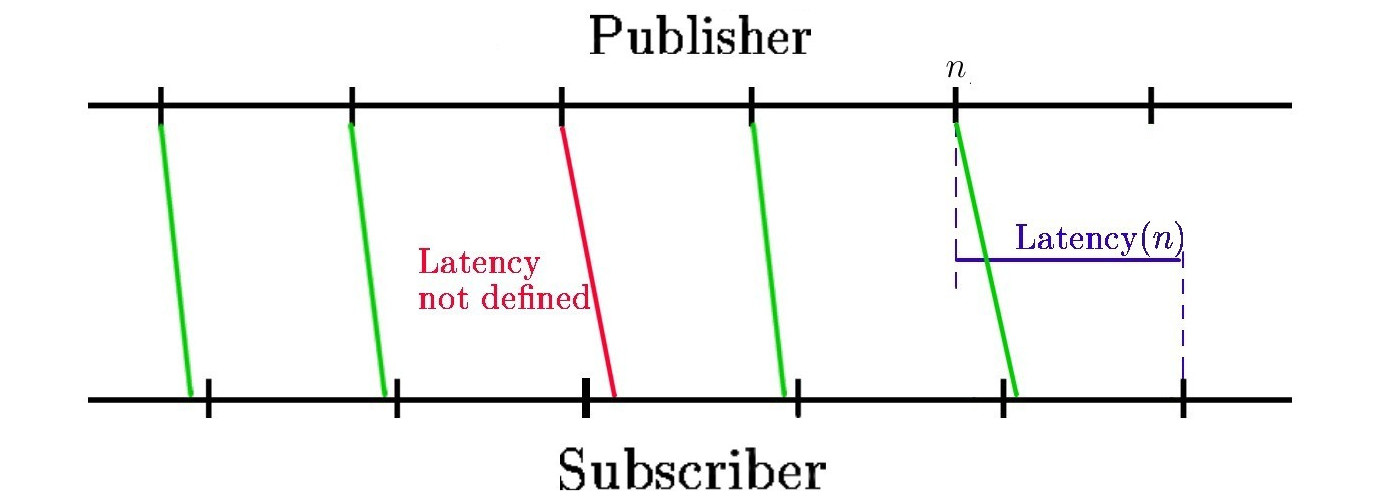
\includegraphics[height=5cm]{latency.jpg}
\caption{Latency definition}\label{latency}
\end{center}
\end{figure}

\begin{defin} \Thmname{Latency}
\[ Latency(n) = c \Big ( min(\{k \in \mathbb{N} | r(n) \leq c(k)\}) \Big ) - s(n) \]
\end{defin}

Since $\forall k, c(k + 1) \leq c(k) + maxT(S)$, we have
$c \big ( min(\{k \in \mathbb{N} | r(n) \leq c(k)\}) \big ) - r(n) \leq maxT(S)$. Therefore,
\begin{thm}\Thmname{Latency bound}
\[ Latency(n) \leq maxT(S) + D \]
\end{thm}

The latency is only defined for a processed message, so this gives little information for assurance properties. However, it can be used to detect a clock failure or a certain type of attack: 
assume for example that the subscriber reads a new message, but the delay since the messages timestamps exceed the latency bound. 
It could be that the clock of one of the nodes drifted significantly from real time, or it may mean that the message had been recorded and was resent later by an attacker.



\subsection{Overtaking}

The model defined in section \ref{ROSarch}, allows an older message to be delivered after a more recent one. We may want to avoid this even if the mailbox system alone doesn't assert that this property holds.
We give here a simple condition that asserts that messages are received in the order they are sent. 

Avoiding overtaking can yield better bounds in some cases to assert other properties are satisfied. By choosing good nodes parameters, a developer can also secure the order of received messages and rely on this to prove correctness of an application.

We have $r(n) \leq s(n) + D$, $s(n) + minT(P) \leq s(n + 1)$ and $s(n + 1) \leq r(n + 1)$. Hence the following theorem:

\begin{thm} \Thmname{Overtaking}
\[ D < minT(P) \quad \implies \quad \forall n \in \mathbb N, \quad r(n) < r(n + 1)\]
\end{thm}


\subsection{Number of lost messages}

As we saw before, messages can be overwritten in the queue before they are actually computed by the subscriber, which means these messages are never processed. However, we can ensure the subscriber does not miss too many consecutive messages

\subsubsection[Consecutive lost messages]{Upper bound for the number of consecutive lost messages}

\begin{defin}\label{consec}
\Thmname{Consecutive lost messages}\\
Formally, we can define the property "the subscriber never misses N consecutive messages" by
\[ \forall k \in \mathbb{N}, \exists l < N, \quad \textrm{\emph{message $k + l$ is processed}}   \]
\end{defin}

First, we have this fundamental lemma:
\begin{lem}\label{existsProcess}
If $c(n) \geq t + D + maxT(P)$, there exists a message $k$ with $t < r(k) \leq c(n)$ that is processed.
\end{lem}

\begin{proof}
$r(0) \leq D < c(n)$. Let $m$ be the maximum of the $l \in \mathbb{N}$ such that $r(l) \leq c(n)$. Since $r(m + 1) > c(n)$, we have $t < r(m) \leq c(n)$.

The set $S = \{l \in \mathbb{N}, t < r(l) \leq c(n)\}$ is finite and nonempty. There exists a $k \in S$ such that $\forall l \in S, r(l) \leq r(k)$. By construction, such a $k$ solves the problem because no message is received between $r(k)$ and the next execution of the subscriber.
\end{proof}

Basic inequality reasoning give this result:

\begin{lem}\label{order_received}
\[ r(m) > s(n) + D - minT(P) \implies n \leq m \]
\[ r(m) < s(n) + minT(P) \implies m \leq n\]
\end{lem}

\begin{thm}\label{clm}\Thmname{Consecutive lost messages}

If $N.minT(P) > 2.D + maxT(S) + maxT(P) - minT(P)$, then the subscriber never misses $N$ consecutive messages.
\end{thm}

\begin{proof}
According to definition~\ref{consec}, given $k \in \mathbb N$, we prove there exists an $l < N$ such that message $k + l$ is processed.

The subscriber executes at least once in every interval of time of length $maxT(S)$. In particular, 
\[ \exists n \in \mathbb N, \quad 
\left\{
\begin{array}{l}
s(k) + 2.D + maxT(P) - minT(P) < c(n) \\
c(n) \leq s(k) + 2.D + maxT(P) - minT(P) + maxT(S)
\end{array} \right. \]

Lemma \ref{existsProcess} gives $\exists l \in \mathbb{N}, s(k) + D - minT(P) < r(l) \leq c(n)$ such that the message $l$ is processed. Since $s(k + N - 1) \geq (N-1) . minT(P)$, with the given condition on $N$, $c(n) < s(k + N - 1) + minT(P)$.

With lemma \ref{order_received}, we have $k \leq l \leq k + N - 1$, and $l$ is processed by construction.
\end{proof}

\paragraph{Case without overtaking :} Assume now that $\forall k \in \mathbb N,\,\, r(k) < r(k + 1)$. In that case, with $m = max({k \in nat, r(k) \leq c(n)})$ we have $r(k) \leq c(n) \implies r(k) \leq r(m)$ which ensures message $m$ is processed.

With $N.minT(P) > D + maxT(S)$, we have $\exists n \in \mathbb N, s(k) + D \leq c(n) < s(k + N)$, then $r(k) \leq c(n) < r(k + N)$. We deduce message $m$ is processed with $k \leq m < k + N$.

\begin{thm}\label{clm2}\Thmname{Consecutive lost messages -- no overtaking}

Assume $N.minT(P) > D + maxT(S)$ and $\forall k \in \mathbb{N},\,\, r(k) < r(k + 1)$. Then the subscriber never misses $N$ consecutive messages.
\end{thm}


\subsubsection{Influence of the queue length}

As one can expect, increasing the message queue size leads to a lower message loss rate. For more comprehension, we first prove this in the case without overtaking. 
Then, we give an idea of the proof in the general case.

Assume we have $\forall k \in \mathbb{N},\,\, r(k) < r(k + 1)$ and we never drop $N$ ($N > 1$) messages with a queue length of $L$. Given $k \in \mathbb N$, there exists $l < N$ such that message $k + l$ is processed. 
If $l < N - 1$, the result is proved. If $l = N - 1$, it means the message $k + N - 1$ was in the queue when some computation $c(n)$ occurred.
With a queue length of $L + 1$, the message $k + N - 2$ was in the queue when $c(n)$ occurred, which means it was processed.

\paragraph{ }
In the general case, we assume the property "never miss $N$ consecutive messages" holds whatever $r$ is as soon as the constraints with $s$ and $D$ are respected (theorem \ref{clm} gives this assurance).
Like in the previous proof, we assume $k + N - 1$ is processed and none of the $k + l$ with $l < N - 1$ is. 
Among non-processed messages received before $r(k + N - 1)$, let $m$ be the one received last. With a queue length of $L + 1$, $m$ is processed with the same argument as before. The difficult part is to prove that this $m$ exists and must be one of the $k + l$, $l < N - 1$.
For this, we construct an other $r'$, consistent with the constraints on $s$ and $D$ but with $N$ consecutive messages lost (which is a contradiction).

Assume that none of the $k+l$ verifies $r(k+l) < r(k+N -1)$. Let $r'$ be a new reception sequence where reception of message $k+N-1$ is delayed to $r(k) + \varepsilon$ (see Figure~\ref{contr}.a),
where $\varepsilon$ is small enough to ensure $r'$ verifies constraints of definition~\ref{reception} and that no message is received between $r'(k)$ and $r'(k+N-1)$.
In this case, messages $k$ to $k+N-2$ are lost because messages that overwrote them with reception $r$ still do with reception $r'$, and message $k+N-1$ is lost because it is received between message $k$ (that is lost) and the next processed message.
This proves $m$ exists and verifies $r(k+l) \leq r(m) < r(k+N-1)$ for some $l$.

Assume $m > k+N-1$. Let $r'$ be the reception sequence where reception of messages $m$ and $k+N-1$ are switched (no change for other messages; see Figure~\ref{contr}.b). $m$ was lost with $r$ means $k+N-1$ is lost with $r'$. Again, messages $k$ to $k+N-1$ are lost with $r'$.

Assume $m < k-1$ (case $m=k-1$ is impossible: $k-1$ must be processed since none of the $k,\dots,k+N-2$ is). If $r(k-1) < r(m)$, switching reception of $k-1$ and $m$ (see Figure~\ref{contr}.c) gives a contradiction with the same argument as previously.
Otherwise, we consider the reception sequence $r'$ where reception of message $k-1$ is anticipated to $r(m)-\varepsilon$. Then, messages $k-1$ to $k+N-2$ are lost (see Figure~\ref{contr}.d).

\begin{figure}[h]
\begin{center}
a) Case $\forall l \in [0, N-2], r(k + l) > r(k+N-1)$ (includes the case where $m$ does not exist)\\
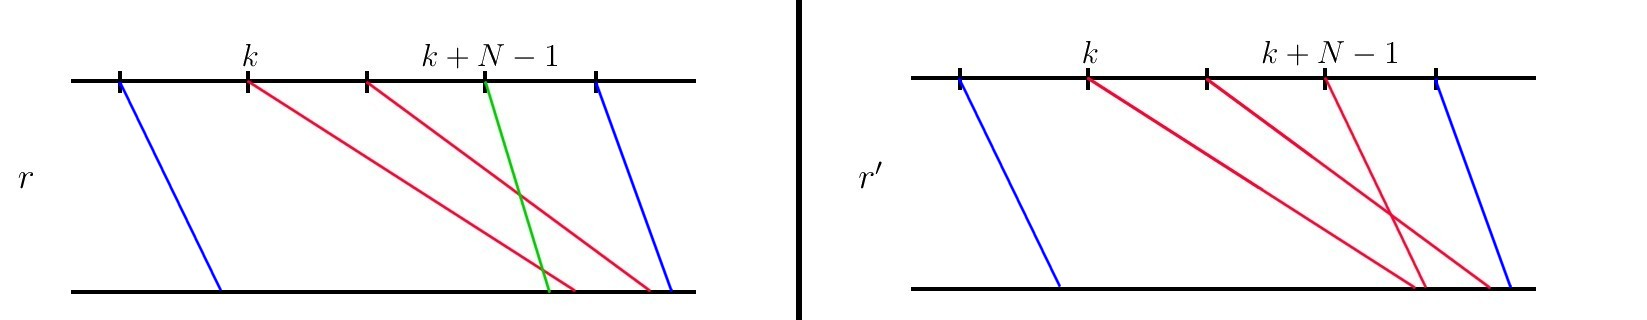
\includegraphics[width=16cm]{contr1.jpg}\\
b) Case $m > k+N-1$\\
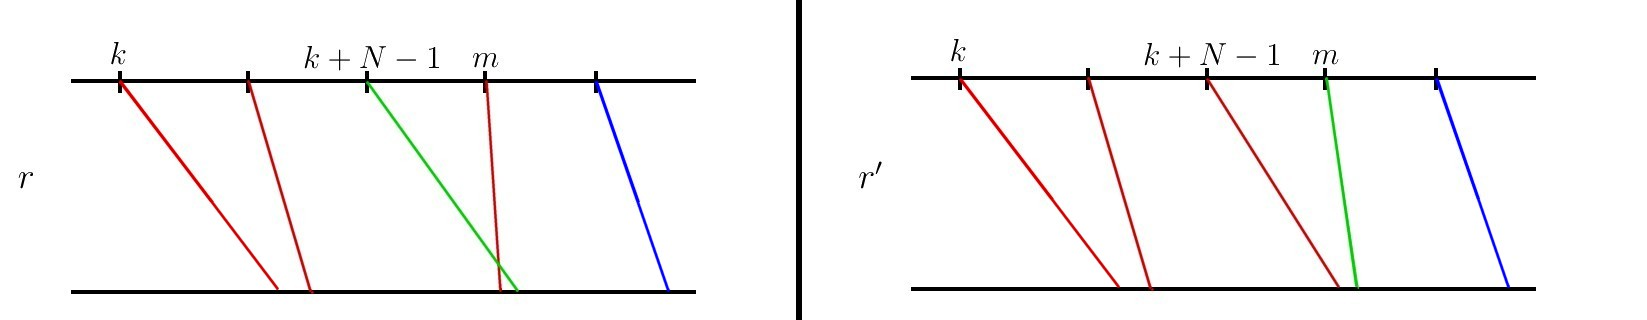
\includegraphics[width=16cm]{contr2.jpg}\\
c) Case $m < k-1$ and $r(m) > r(k-1)$\\
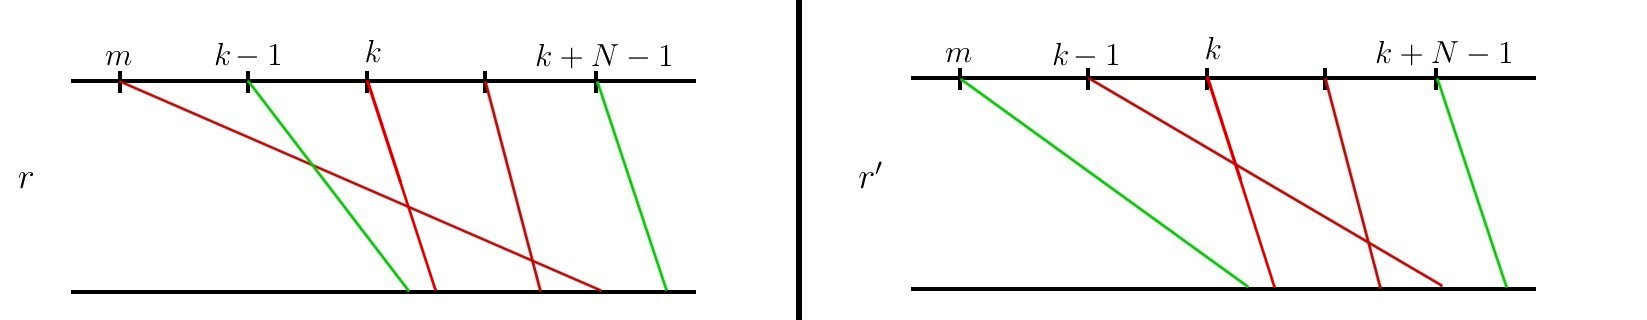
\includegraphics[width=16cm]{contr3.jpg}\\
d) Case $m < k-1$ and $r(m) < r(k-1)$\\
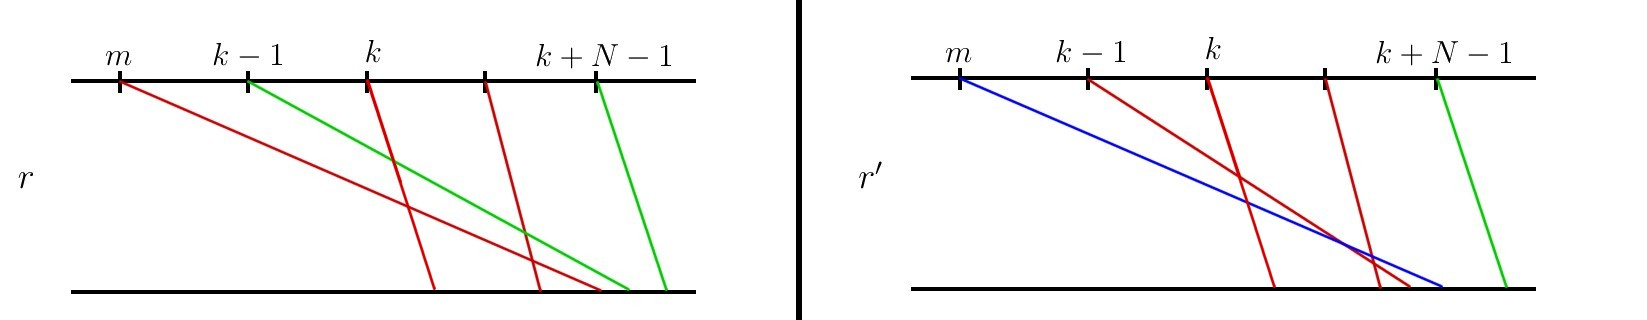
\includegraphics[width=16cm]{contr4.jpg}\\
(green: processed -- red: lost -- blue: status unknown/irrelevant)
\caption{Getting contradictions}\label{contr}
\end{center}
\end{figure}

\paragraph{ }By a simple induction, we then get the following result:

\begin{thm} 
Let $N$ satisfies conditions of either theorem~\ref{clm} or theorem~\ref{clm2}. Let $m < N$ and assume $L > m$. Then the subscriber never miss $N - m$ consecutive messages.

In particular, if $L \geq N$, no message is lost.
\end{thm} 

\subsection{Age of processed messages}

In this section, we prove that at each computation, the subscriber gets (from a newly received message or with a backup from previous computation) a reasonably recent message.

This is essentially a bound on the age of processed messages that will be used in next sections to prove end-to-end properties. It is also helpful to detect errors: when the latest available message to the subscriber is older than the bound, it can raise a timeout flag. By collecting these flags, a monitor could guess whether the publisher node crashed or there is a network failure.

\subsubsection{Definition and basic properties}

The aim is to model the following behavior (see Figure~\ref{age}):
 At each computation, if messages are available in the queue, the node chooses the most recent one and saves it to give a backup solution for next computation. 
If not, it uses the backup given by previous step (while no message has been received, and no backup is available, a default value -- set at initialization time -- is used)

\begin{figure}[h]
\begin{center}
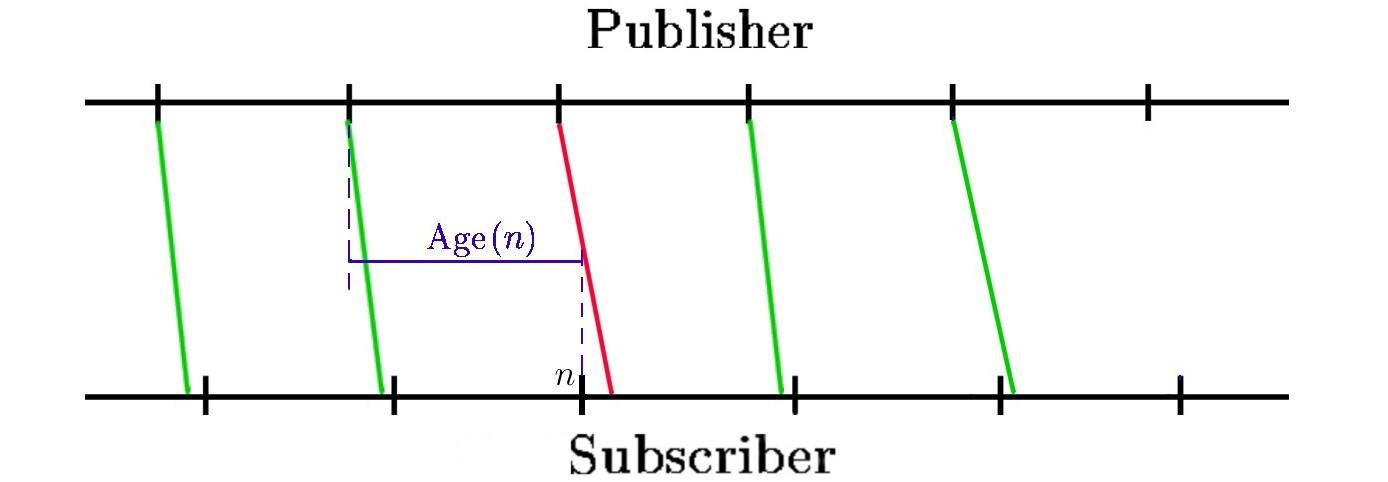
\includegraphics[height=5cm]{age.jpg}
\caption{Age definition}\label{age}
\end{center}
\end{figure}


\vbox{
\begin{defin}\label{ageDef}\Thmname{Age for the most recent available message}

For $n \neq 0$, we define the (finite, but maybe empty) set of messages computed at step n by
\[PL(n) = \big \{k \in \mathbb{N}, c(n - 1) < r(k) \leq c(n) 
\wedge \textrm{\emph{message $k$ is processed}} \big \}\]

Then, the age of the most recent available message can be defined by the recursive function \\
\emph{\texttt{Age($n$) = \{\\
\indent if $n=0$ then 0 \\
\indent else \{if $PL(n) = \emptyset$\\
\indent\indent then \{Age($n - 1$)$ + c(n) - c(n-1)$\}\\
\indent\indent else \{$c(n) - s(max(PL(n))$\}\\
\}\}
}}
\end{defin}
}

\vbox{
\begin{lem}\label{ageLem}
A simple induction over $n$ gives \texttt{\emph{Age}($n$)}$\leq c(n)$. 

Also, with the same argument as in the proof of lemma~\ref{existsProcess}, we have:
\[PL(n) = \emptyset \,\, \Longleftrightarrow \,\, 
\{k \in \mathbb{N}, c(n - 1) < r(k) \leq c(n)\} = \emptyset
\]
\end{lem}
}

\subsubsection{Upper bound in worst case scenario}

\begin{thm}\label{maxAge}\Thmname{Age bound}
\[ \texttt{\emph{Age($n$)}} < 2.D + maxT(P) \]
\end{thm}

\begin{proof}
First, we see by a simple induction over n that:
\[r(k) \leq c(n) \implies \texttt{Age($n$)} \leq c(n) - r(k) + D\]
(if $PL(n) = \emptyset$, lemma~\ref{ageLem} gives $r(k) \leq c(n-1)$. Otherwise, using the definition of a processed message, we either have $r(k) \leq r(max(PL(n)))$ or $k \leq max(PL(n))$. In both cases, \mbox{$s(max(PL(n))) \geq r(k) - D$})

In the case $c(n) \leq D + maxT(P)$, lemma~\ref{ageLem} gives the result. Otherwise, by lemma~\ref{existsProcess}, there exists a message $k$ such that $c(n) - D - maxT(P) < r(k) \leq c(n)$, which proves the theorem with the property above.
\end{proof} 

When messages are delivered in the same order they were sent, we get a better bound:

\begin{thm}\label{maxAge2}\Thmname{Age bound -- no overtaking}
\[ \forall k \in \mathbb{N},\,\, r(k) < r(k+1) \quad \implies \quad
\texttt{\emph{Age($n$)}} < D + maxT(P) \]
\end{thm}

\begin{proof}
When no overtaking is possible, the message $m(n) = max(\{k\in \mathbb{N},\, r(k) \leq c(n)\})$ (assuming the considered set is non empty) is processed. 

Since $r(m(n)+1) \leq s(m(n)) + D + maxT(P)$, we have 
\[ c(n) - D -maxT(P) < s(m(n)) \leq c(n) \]

$r(m(n)) \leq c(n-1) \implies m(n) = m(n-1)$. Therefore, we get by induction 
\[ \texttt{Age($n$)} = 
\left\{ \begin{array}{ll}
c(n) - m(n) &\textrm{ if $ r(0) \leq c(n)$}\\
c(n) &\textrm{ if $ r(0) > c(n)$, which means $c(n) < D$}
\end{array}\right.
\]
\end{proof}


